\chapter{Calculation of Condensed Field}

\section{Relating Fluid and Pion Fields}

The signature is $(-,+,+,+)$.

Start with the Lagrangian of the linear $\sigma$-model for the real-valued $O(4)$-vector $\varphi_a=(\sigma,\mathbf{\pi})$.
\begin{equation}
    \mathscr{L}=-\frac{1}{2}\partial_\mu\sigma\partial^\mu\sigma-\frac{1}{2}\partial_\mu\mathbf{\pi}\partial^\mu\mathbf{\pi}-\frac{1}{2}m^2(\sigma^2+\mathbf{\pi}^2)-\frac{\lambda}{4}(\sigma^2+\mathbf{\pi}^2)^2-\epsilon\sigma
\end{equation}
and from \ref{subsubsec:linearsigmamodel} we find, that if $m^2=-\mu^2<0$ SSB occurs (plus, $\epsilon\neq 0$ explicitly breaks the symmetry) with the VEV $v$ and masses of the $\sigma$ and $\mathbf{\pi}$ excitation in $\varphi_a=(v+\delta\sigma,\mathbf{\pi})$ are given by (note the difference in conventions $\lambda\to 6\lambda$ w.r.t. \ref{subsubsec:linearsigmamodel})
\begin{equation}
    \left\{
    \begin{split}
        v_0         & =\frac{\mu}{\sqrt{\lambda}}+\epsilon\frac{1}{2\mu^2}+\mathcal{O}(\epsilon^2) \\
        m_\sigma^2 & =2\mu^2+\mathcal{O}(\epsilon)                                                \\
        m_\pi^2    & =\epsilon\frac{\sqrt{\lambda}}{\mu}+\mathcal{O}(\epsilon^2)
    \end{split}
    \right.\qquad\overset{\text{to lowest order}}{\iff}\qquad
    \left\{
    \begin{split}
        \mu&=\frac{m_\sigma}{\sqrt{2}}\\
        \lambda&=\frac{m_\sigma^2}{2v_0^2}\\
        \epsilon&=v_0m_\pi^2
    \end{split}
    \right.
    \label{eq:LinearSigmaModel_CouplingsMassesRelation}
\end{equation}
Choose now a fixed alignment of the condensate $\mathbf{\pi}=\pi\mathbf{e}$ with $\mathbf{e}\cdot\mathbf{e}=1$ determining the orientation in isospin space. This choice breaks $O(4)$ to $O(2)$ (we restrict ourselves to $SO(2)$) and use to isomorphism $SO(2)\overset{\sim}{=}U(1)$ to write the linear $\sigma$-model as a theory of a complex scalar field $\phi=\frac{1}{\sqrt{2}}(\sigma+\imagu\pi)=\rho e^{\imagu\vartheta}$.
\begin{subequations}
    \begin{align}
        \text{in terms of}\,(\phi,\phi^*)      &  & \mathscr{L} & =-(\partial_\mu\phi)(\partial^\mu\phi^*)+\mu^2\phi\phi^*-\frac{\lambda}{2}(\phi\phi^*)^2+\frac{\epsilon}{\sqrt{2}}(\phi+\phi^*)                                   \\
        \text{in terms of}\,(\rho,\vartheta^*) &  & \mathscr{L} & =-(\partial_\mu\rho)(\partial^\mu\rho)-\rho^2(\partial_\mu\vartheta)(\partial^\mu\vartheta)+\mu^2\rho^2-\frac{\lambda}{2}\rho^4+\sqrt{2}\epsilon\rho\cos\vartheta
    \end{align}
\end{subequations}
The classical equations of motion arising from this are
\begin{subequations}
    \begin{align}
        \text{in terms of}\,(\phi,\phi^*)      &                                                                                                                           & -\Box\phi                                  & =(\partial_t^2-\mathbf{\nabla}^2)\phi=\big[\mu^2-\lambda(\phi^*\phi)\big]\phi+\frac{\epsilon}{\sqrt{2}} \\
        \text{in terms of}\,(\rho,\vartheta^*) &                                                                                                                           &
        -\Box\rho                              & =\big[-(\partial_\mu\vartheta)(\partial^\mu\vartheta)+\mu^2-\lambda\rho^2\big]\rho+\frac{\epsilon}{\sqrt{2}}\cos\vartheta                                                                                                                                                        \\
                                               &                                                                                                                           & -\partial_\mu(\rho^2\partial^\mu\vartheta) & =-\frac{\epsilon}{\sqrt{2}}\rho\sin\vartheta
    \end{align}
\end{subequations}
The conserved Noether current of thse symmetry $\theta\to\theta+\alpha$ (in the limit $\epsilon\to 0$) and energy-momentum tensor are
\begin{subequations}
    \begin{align}
        \alpha j^\mu & =-\frac{\partial\mathscr{L}}{\partial(\partial_\mu\vartheta)}\delta\vartheta=2\alpha\rho^2(\partial^\mu\vartheta)                                                                                                                                                             \\
        T^{\mu\nu}   & =\frac{2}{\sqrt{-g}}\frac{\delta(\sqrt{-g}\mathscr{L})}{\delta g_{\mu\nu}}=2\frac{2\partial\mathscr{L}}{\partial g_{\mu\nu}}+g^{\mu\nu}\mathscr{L}=2\big[(\partial^\mu\rho)(\partial^\nu\rho)+\rho^2(\partial^\mu\vartheta)(\partial^\nu\vartheta)\big]+g^{\mu\nu}\mathscr{L}
    \end{align}
\end{subequations}
where $\delta\sqrt{-g}=\frac{-1}{2\sqrt{-g}}\delta g=\frac{-1}{\sqrt{-g}}gg^{\mu\nu}\delta g_{\mu\nu}=\frac{\sqrt{-g}}{2}g^{\mu\nu}\delta g_{\mu\nu}$ was used.

In a tree-level approximation one only needs to solve the classical equations of motion. In the limit $\epsilon\to 0$ a valid solution is
\begin{equation}
    \partial_\mu\vartheta=\const\,,\qquad\rho=\sqrt{\frac{\chi^2+\mu^2}{\lambda}}+\mathcal{O}(\epsilon)\qquad(\chi^2\defeq-(\partial_\mu\vartheta)(\partial^\mu\vartheta))
\end{equation}
We might generalize the solution to the case $\partial_\mu\vartheta\approx\const$ which should be valid in the limit $\chi^2\ll\mu^2=\frac{m_\sigma^2}{2}$. On these solutions one finds
\begin{subequations}
    \begin{align}
        \mathscr{L}\big\vert_{\text{EOM}} & =\rho^2(\chi^2+\mu^2-\frac{\lambda}{2}\rho^2)=\rho^2\frac{\chi^2+\mu^2}{2}                    \\
        T^{\mu\nu}\big\vert_{\text{EOM}}  & =2\rho^2(\partial^\mu\vartheta)(\partial^\nu\vartheta)+g^{\mu\nu}\rho^2\frac{\chi^2+\mu^2}{2}
    \end{align}
\end{subequations}

Assume the dynamics of the field could be described by ideal hydrodynamics, i.e. a conserved current and energy-momentum tensor of the form \todo{I really don't know about the signature}
\begin{subequations}
    \begin{align}
        j^\mu      & =n_s\nu^\mu\qquad(v^\mu v_\mu=-1)          \\
        T^{\mu\nu} & =(\epsilon_s+P_s)v^\mu v^\nu+g^{\mu\nu}P_s
    \end{align}
\end{subequations}
from which the prefactors can be extracted by the contractions
\begin{equation}
    n_s=\sqrt{-j^\mu j_\mu}\,,\qquad\epsilon_s=v_\mu v_\nu T^{\mu\nu}\,,\qquad P_s=\frac{1}{3}(g_{\mu\nu}+v_\mu v_\nu)T^{\mu\nu}
\end{equation}

Identifying the field theoretic with the hydrodynamic viewpoint it immediately follows that
\begin{subequations}
    \begin{gather}
        n_s=2\rho^2\chi\,,\qquad v^\mu=\chi^{-1}(\partial^\mu\vartheta)\qquad(\iff\chi=-v^\mu(\partial_\mu\vartheta))\\
        \epsilon_s=2\rho^2\chi^2-\rho^2\frac{\chi^2+\mu^2}{2}=\rho^2\frac{4\chi^2-(\chi^2+\mu^2)}{2}=\frac{(\chi^2+\mu^2)(3\chi^2-\mu^2)}{2\lambda}
    \end{gather}
\end{subequations}

% \textcolor{red}{\textbf{NOTE THE HANDWRITTEN NOTES SEEM TO HAVE MOSTLY $(+,-,-,-)$ SIGNATURE EXCEPT FOR THE CLAIM $v_\mu v^\mu=-1$, WHIS IS SIMPLY INCONSISTENT}}
% 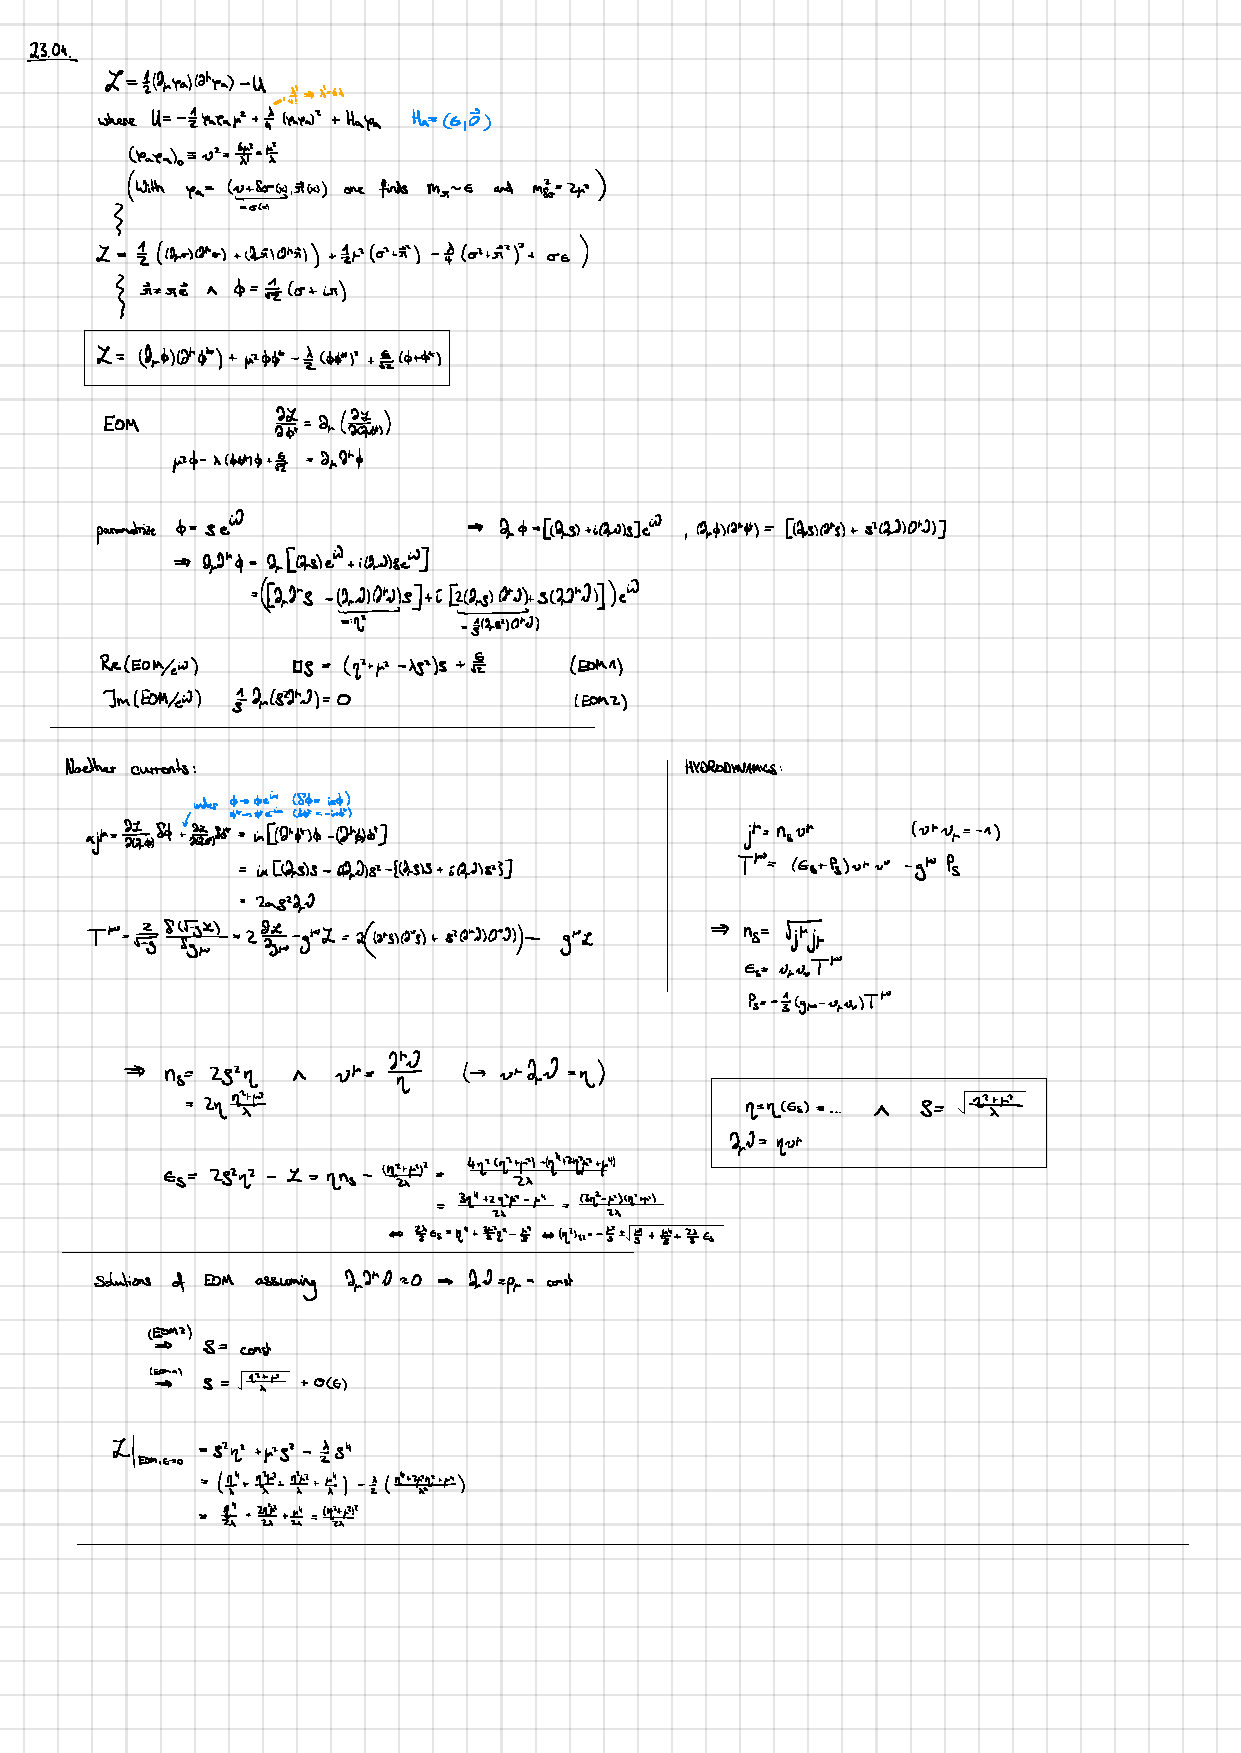
\includepdf{resources/notes_0423.pdf}

\paragraph*{How to apply this?}\mbox{}\\

The freeze-out surface is invariant under rotations (= independent of polar angle $\varphi$) around the collision axis and longitudinal boosts (= independent of rapidity $\eta_s$) and hence parametrized by a one-dimensional curve in the $r\text{-}\tau$-plane. The curve itself may be parametrized by some real parameter $\alpha$, following some mapping $\alpha\mapsto (r(\alpha),\tau(\alpha))$. From the hydro simulation we wish to identify the gradient $\partial_\mu\vartheta\sim u_\mu$ of the complex phase of the condensate field with the fluid $4$-velocity $u_\mu$, hence in order to find the phase of the field, an integration of $\partial_\mu\vartheta$ over the hypersurface is needed and an integration constant $\vartheta_0$ can be chosen freely. Choose $\alpha=\arctan(\tau/r)$ to be the polar angle of the point $(r(\alpha),\tau(\alpha))$ in the $r\text{-}\tau$-plane. Since $r,\tau>0$ $\alpha$ is restricted to the range $[0,\pi]$ and $\vartheta(\alpha)$ on the hypersurface can be calculated via
\begin{equation}
    \vartheta(\alpha)=\vartheta_0+\int_0^\alpha\dt s\frac{\dt\vartheta}{\dt s}=\vartheta_0+\int_0^\alpha\dt s\frac{\partial x^\mu(s)}{\partial s}\partial_\mu\vartheta
\end{equation}
$\partial x^\mu(s)/\partial s$ represents the tangent vector of the freeze-out surface.

The energy density $\epsilon$ and $4$-velocity $u^\mu$ of the fluid is related to the condensate phase and density via
\begin{subequations}
    \begin{gather}
        -(\partial_\mu\vartheta)(\partial^\mu\vartheta)=\chi^2=\frac{-\mu^2+\sqrt{6\epsilon\lambda+4\mu^4}}{3}\\
        \partial^\mu\vartheta=\chi u^\mu\,,\qquad\rho^2=\sqrt{\frac{\chi^2+\mu^2}{\lambda}}
    \end{gather}
\end{subequations}
One may use the relations \eqref{eq:LinearSigmaModel_CouplingsMassesRelation} to rewrite the above equation in terms of the particle masses and the $\sigma$-vev $v_0$.
\begin{equation}
    \chi^2=\frac{-m_\sigma^2/2+\sqrt{3\epsilon m_\sigma^2/v_0^2+m_\sigma^4}}{3}=\frac{-m_\sigma^2+2m_\sigma\sqrt{3\epsilon/v_0^2+m_\sigma^2}}{6}\,,\qquad\rho=\sqrt{v_0\frac{2\chi^2+m_\sigma^2}{m_\sigma^2}}
\end{equation}
\todo{This is a number of order $m_{\Sigma}^2$. Of what order is $u_\mu$ (in $\text{eV}^{-1}$? But then again, isn't $u^\mu$ normalized to $\pm 1$?)}

In Milne coordinates $(x^\mu)=(\tau,r,\varphi,\eta_s)$ the $4$-velocity has components $(u^\mu)=(\gamma,\gamma v,0,0)$, where $v=v(\alpha)$ is a function on the freeze-out surface. \todo{Are these upstairs or downstairs indexed coordinates?}

\section{Finding the Spectrum at the Detector Surface}

In general the particle number $N$ and particle number density $n(\vec{x})$ in position space and $n(\vec{p})$ in momentum space associated to the condensate $\phi(\vec{x})$ of a complex scalar field are given by the relations
\begin{subequations}
    \begin{gather}
        n(\vec{x})=\phi(\vec{x})\phi^*(\vec{x})\,,\qquad n(\vec{p})=\phi(\vec{p})\phi^*(\vec{p})\\
        N=\int\dt^3xn(\vec{x})=\int\frac{\dt^3p}{(2\pi)^3}n(\vec{p})
    \end{gather}
\end{subequations}
with the convention $\phi(\vec{x})=\int\dt^3p/(2\pi)^3\phi(\vec{p})e^{-\imagu\vec{p}\vec{x}}$ for the Fourier transform.


% The field configuration found by this translation prescription is then propagated forwards in time by means of the retarded Greens function
% \begin{equation}
%     \overline{\phi}(x)=\langle\phi_a(x)\rangle=\int\dt^dyG_{\text{ret}}(x,y)j(y)
% \end{equation}
% $j(y)$ is defined to be the field configruation on the freezout surface. The retarded Greens function is given by $G_{\text{ret}}(x,y)=\Theta(x^0-y^0)\big(D(x-y)-D(y-x)\big)$ where
% \begin{equation}
%     D(\Delta x)=\int\frac{\dt^3p}{(2\pi)^3}\frac{1}{2\omega_\vec{p}}e^{-\imagu(\omega_\vec{p}\Delta t-\vec{p}\Delta\vec{x})}
% \end{equation}
% and $\omega_\vec{p}=\sqrt{m^2+\vec{p}^2}$.

% 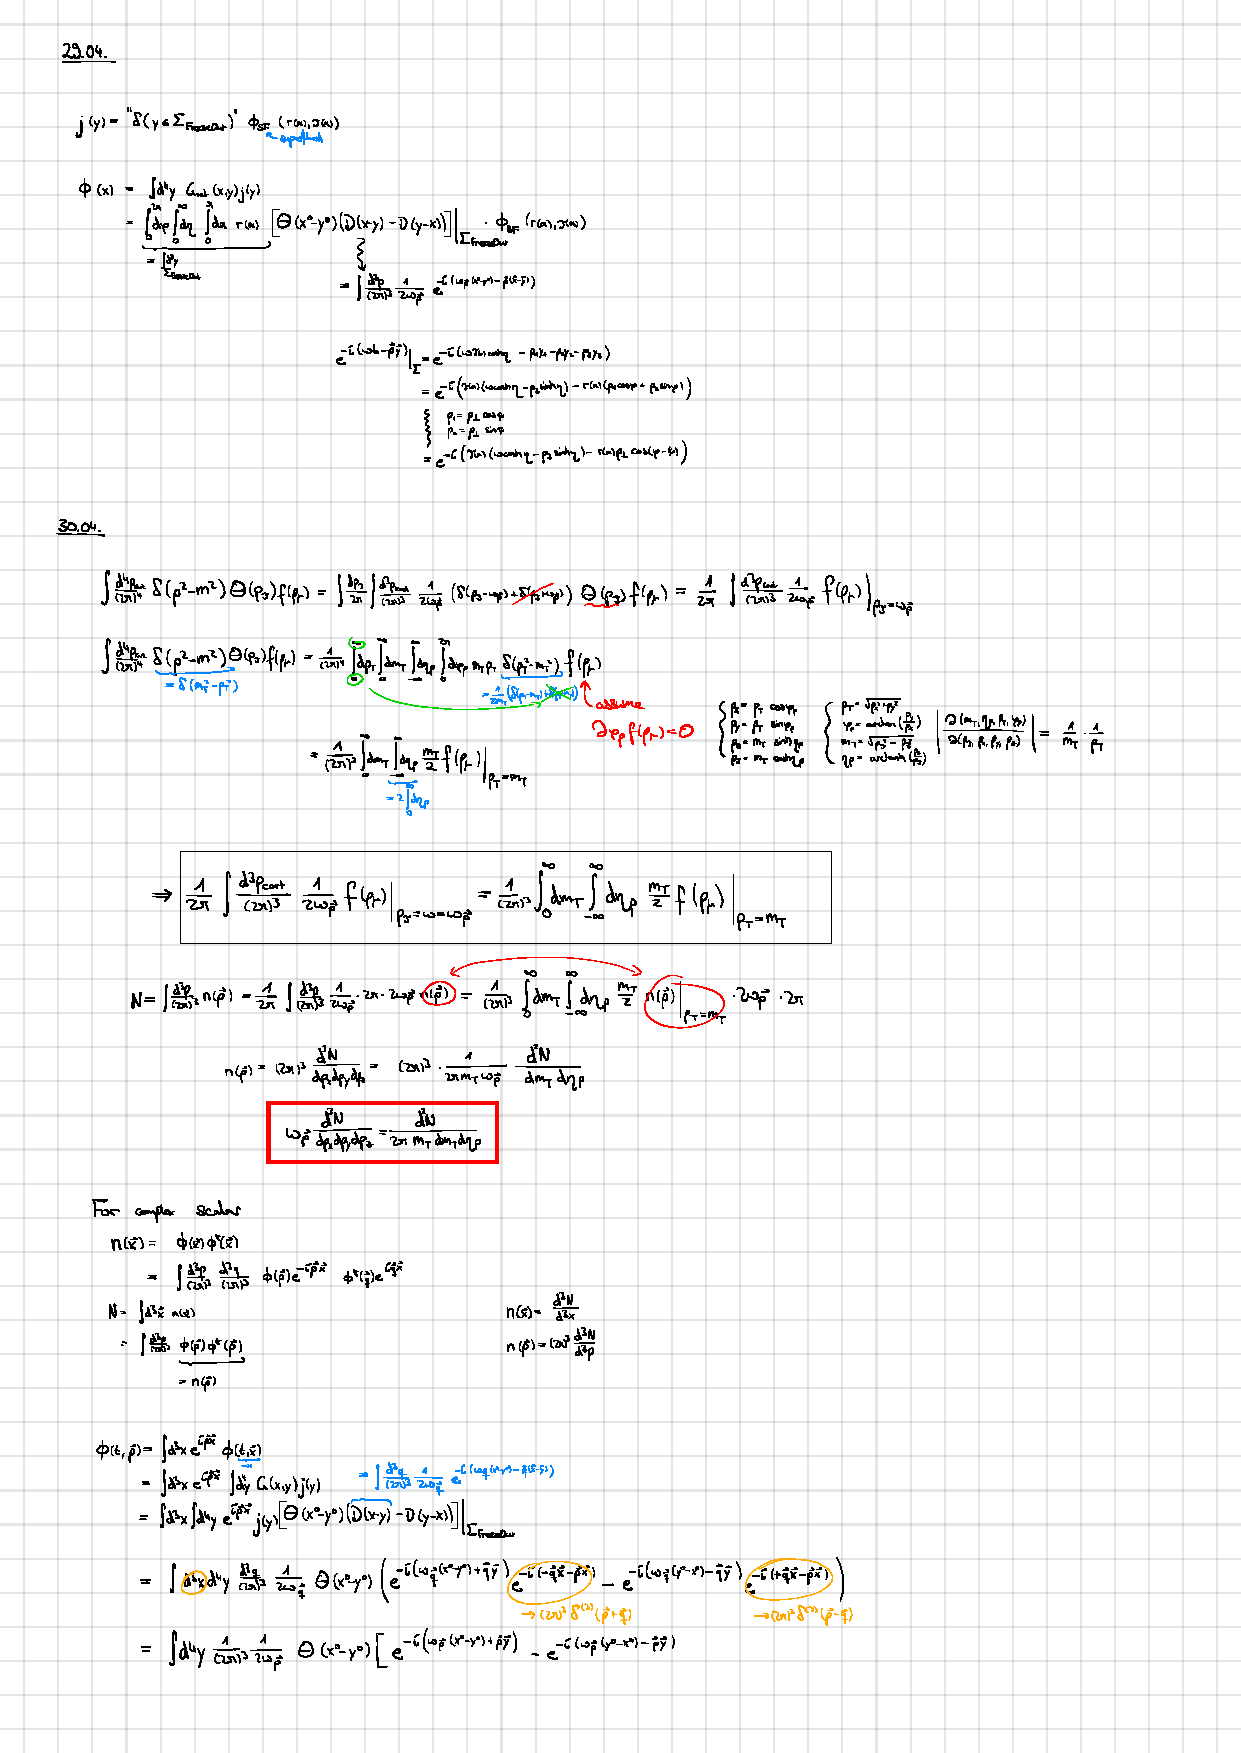
\includepdf{resources/notes_0430.pdf}

\subsection{Treating the Freeze Out Field as Source Term???}

Let's evaluate the Fourier transform of the condensate field. The calculation uses the result from linear response theory for the deviation of the expectation value $\overline{\phi}$ induced by a source term $j$, which we for the moment we assume to be specified by the hydro variables on the freezeout surface.
\begin{subequations}
    \begin{equation}
        \overline{\phi}(x)\equiv\langle\phi(x)\rangle=\int\dt^4G_{\text{ret}}(x,y)j(y)
    \end{equation}
    The retarded Greens function is given by
    \begin{equation}
        G_{\text{ret}}(x,y)=\Theta(x^0-y^0)\big[D(x-y)-D(y-x)\big]
    \end{equation}
    with the propagator
    \begin{equation}
        D(x-y)=\int\frac{\dt^3q}{(2\pi)^3}\frac{e^{-\imagu[\omega_{\vec{q}}(x^0-y^0)-\vec{q}(\vec{x}-\vec{y})]}}{2\omega_{\vec{q}}}
    \end{equation}
    and the relations
    \begin{equation}
        \int\dt^3x e^{\imagu\vec{x}(\vec{p}-\vec{q})}=(2\pi)^3\delta^{(3)}(\vec{p}-\vec{q})\,,\qquad\phi(t,\vec{p})=\int\dt^3x e^{\imagu\vec{p}\vec{x}}\phi(t,\vec{x})
    \end{equation}
\end{subequations}
Putting things together
\begin{subequations}
    \begin{align}
        \overline{\phi}(x^0\equiv t,\vec{p}) & =\int\dt^3x e^{\imagu\vec{p}\vec{x}}\overline{\phi}(x^0\equiv t,\vec{x})                                                                                                                                                                                                                                                           \\
                                             & =\int\dt^3xe^{\imagu\vec{p}\vec{x}}\int\dt^4yG_{\text{ret}}(x,y)j(y)                                                                                                                                                                                                                                                               \\
                                             & =\int\dt^3xe^{\imagu\vec{p}\vec{x}}\int\dt^4y\Theta(x^0-y^0)\big[D(x-y)-D(y-x)\big]j(y)                                                                                                                                                                                                                                            \\
                                             & =\int\dt^3xe^{\imagu\vec{p}\vec{x}}\int\dt^4y\int\frac{\dt^3q}{(2\pi)^3}\frac{1}{2\omega_{\vec{q}}}\Theta(x^0-y^0)\times\nonumber                                                                                                                                                                                                  \\
                                             & \phantom{=}\qquad\times\big[e^{-\imagu[w_{\vec{q}}(x^0-y^0)-\vec{q}(\vec{x}-\vec{y})]}-e^{\imagu[w_{\vec{q}}(x^0-y^0)-\vec{q}(\vec{x}-\vec{y})]}\big]j(y)                                                                                                                                                                          \\
                                             & =\int\dt^3x\int\dt^4y\int\frac{\dt^3q}{(2\pi)^3}\frac{1}{2\omega_{\vec{q}}}\Theta(x^0-y^0)\times\nonumber                                                                                                                                                                                                                          \\
                                             & \phantom{=}\qquad\times\big[e^{-\imagu[w_{\vec{q}}(x^0-y^0)+\vec{q}\vec{y}]}e^{\imagu(\vec{p}+\vec{q})\vec{x}}-e^{\imagu[w_{\vec{q}}(x^0-y^0)+\vec{q}\vec{y}]}e^{\imagu(\vec{p}-\vec{q})\vec{x}}\big]j(y)                                                                                                                          \\
                                             & =\int\dt^4y\int\dt^3q\frac{1}{2\omega_{\vec{q}}}\Theta(x^0-y^0)\times\nonumber                                                                                                                                                                                                                                                     \\
                                             & \phantom{=}\qquad\times\big[e^{-\imagu[w_{\vec{q}}(x^0-y^0)+\vec{q}\vec{y}]}\delta^{(3)}(\vec{p}+\vec{q})-e^{\imagu[w_{\vec{q}}(x^0-y^0)+\vec{q}\vec{y}]}\delta^{(3)}(\vec{p}-\vec{q})\big]j(y)                                                                                                                                    \\
                                             & =\int\dt^4y\frac{1}{2\omega_{\vec{p}}}\Theta(x^0-y^0)\big[e^{-\imagu[w_{\vec{p}}(x^0-y^0)-\vec{p}\vec{y}]}-e^{\imagu[w_{\vec{p}}(x^0-y^0)+\vec{p}\vec{y}]}\big]j(y)                                                                                                                                                                \\
                                             & =\int\dt^4y\frac{1}{2\omega_{\vec{p}}}\Theta(x^0-y^0)e^{\imagu\vec{p}\vec{y}}\big[e^{-\imagu\omega_{\vec{p}}(x^0-y^0)}-e^{\imagu\omega_{\vec{p}}(x^0-y^0)}\big]j(y)                                                                                                                                                                \\
                                             & =\int\dt^4y\frac{1}{\imagu\omega_{\vec{p}}}\Theta(x^0-y^0)e^{\imagu\vec{p}\vec{y}}\sin(\omega_{\vec{p}}(x^0-y^0))j(y)                                                                                                                                                                                                              \\
        \intertext{Specify this for the relevant case $\text{supp}j=\Sigma_{\text{freeze-out}}$ and parametrize the integral over the hypersurface $\Sigma$ via (see \eqref{calc:HypersurfaceMetric})$\int_\Sigma\dt^3\Sigma=\int\dt\varphi\dt\eta\dt\alpha r(\alpha)\tau(\alpha)\sqrt{r^{\prime 2}(\alpha)-\tau^{\prime 2}(\alpha)}$}
        \overline{\phi}(x^0\equiv t,\vec{p}) & =\int_0^{2\pi}\dt\varphi\int_{-\infty}^\infty\dt\eta\int_0^\pi\dt\alpha r(\alpha)\tau(\alpha)\sqrt{r^{\prime 2}(\alpha)-\tau^{\prime 2}(\alpha)}\frac{1}{\imagu\omega_{\vec{p}}}\Theta(x^0-\tau(\alpha)\cosh\eta)\times                                                                                                  \nonumber \\
                                             & \phantom{=}\qquad\times\exp\left(\imagu[\vec{p}_\perp\vec{x}_\perp+p_z\tau(\alpha)\sinh\eta]\right)\sin(\omega_{\vec{p}}(x^0-\tau(\alpha)\cosh\eta))j(\tau(\alpha),r(\alpha))                                                                                                                                                      \\
        \intertext{Performing the $\varphi$-integration, with $\varphi$ appearing in the integrand in $\vec{x}_\perp=(r\cos\varphi,r\sin\varphi)$, we choose to align $\varphi=0$ with the $p_x$ direction. Then $\vec{p}_\perp\vec{x}_\perp=p^\perp r\cos\varphi$. Use the Bessel function $J_0$ of first kind to simplify}
        \overline{\phi}(x^0\equiv t,\vec{p}) & =\int_{-\infty}^\infty\dt\eta\int_0^\pi\dt\alpha r(\alpha)\tau(\alpha)\sqrt{r^{\prime 2}(\alpha)-\tau^{\prime 2}(\alpha)}\frac{1}{\imagu\omega_{\vec{p}}}\Theta(x^0-\tau(\alpha)\cosh\eta)\times                                                                                                  \nonumber                        \\
                                             & \phantom{=}\qquad\times 2\pi J_0(p^\perp r(\alpha))\exp\left(\imagu p_z\tau(\alpha)\sinh\eta\right)\sin(\omega_{\vec{p}}(x^0-\tau(\alpha)\cosh\eta))j(\tau(\alpha),r(\alpha))
    \end{align}
\end{subequations}

\begin{calc}[Metric on Hypersurface]{calc:HypersurfaceMetric}
    Recall the metric $g_{\mu\nu}=\text{diag}(-1,1,\tau^2,r^2)$ in coordinates $(\tau,r,\eta,\varphi)$. Orthonormal tangent vectors to the freeze out hypersurface are $(\hat\partial_\varphi)^\mu=(0,0,0,r^{-1})=r^{-1}(\partial_\varphi)^\mu$, $(\hat\partial_\eta)^\mu=(0,0,\tau^{-1},0)=\tau^{-1}(\partial_\eta)^\mu$ and $(\hat\partial_\alpha)^\mu=\sqrt{r^{\prime 2}(\alpha)-\tau^{\prime 2}(\alpha)}^{-1}(\tau^{\prime}(\alpha),r^{\prime}(\alpha),0,0)=D(\alpha)(\partial_\alpha)^\mu$ with $D(\alpha)=\sqrt{r^{\prime 2}(\alpha)-\tau^{\prime 2}(\alpha)}^{-1}$. The projector on the hypersurface is
    \begin{equation}
        \gamma_{\mu\nu}=(\hat\partial_\varphi)_\mu(\hat\partial_\varphi)_\nu+(\hat\partial_\eta)_\mu(\hat\partial_\eta)_\nu+(\hat\partial_\alpha)_\mu(\hat\partial_\alpha)_\nu=\begin{pmatrix}
            D^2(\alpha)\tau^{\prime2}(\alpha)               & -D^2(\alpha)\tau^\prime(\alpha)r^\prime(\alpha) & 0      & 0   \\
            -D^2(\alpha)\tau^\prime(\alpha)r^\prime(\alpha) & D^2(\alpha)r^{\prime2}(\alpha)                  & 0      & 0   \\
            0                                               & 0                                               & \tau^2 & 0   \\
            0                                               & 0                                               & 0      & r^2
        \end{pmatrix}
    \end{equation}
    The normal of the hypersurface is $n^\mu\equiv(\hat\partial_\alpha^\perp)^\mu=D(\alpha)(r^\prime(\alpha),\tau^\prime(\alpha),0,0)$ and is timelike where $D$ is real. Naturally $\gamma_{\mu\nu}n^\nu=0$. In the basis $(\partial_\alpha,\partial_\eta,\partial_\varphi,n)$ using (in short form)
    \begin{equation}
        (\partial_\alpha)^\nu\gamma_{\mu\nu}(\partial_\alpha)^\mu=\begin{pmatrix}
            \tau^\prime \\r^\prime
        \end{pmatrix}^T\begin{pmatrix}
            -\tau^\prime \\
            r^\prime
        \end{pmatrix}=D^{-2}
    \end{equation}
    the hypersurface metric in coordinates $x^i=(\alpha,\eta,\varphi)$ reads
    \begin{equation}
        \gamma_{ij}=\text{diag}(D^{-2}(\alpha),\tau^2(\alpha),r^2(\alpha))
    \end{equation}
    and the volume element is given by $\dt\Sigma=r(\alpha)\tau(\alpha) D^{-1}(\alpha)\dt\alpha\dt\eta\dt\varphi$. The oriented surface element is \begin{equation}
        \dt\Sigma^\mu=n^\mu\dt\Sigma=r(\alpha)\tau(\alpha)(r^\prime(\alpha),\tau^\prime(\alpha),0,0)\dt\alpha\dt\eta\dt\varphi
    \end{equation}
\end{calc}

\subsection{Converting Spectra between Coordinate Systems}

Consider the coordinate change in momentum space
\begin{equation}
    \left\{
    \begin{split}
        p_x&=p^\perp\cos\varphi_p\\
        p_y&=p^\perp\sin\varphi_p\\
        p_z&=m^\perp\sinh\eta_p\\
        p_t&=m^\perp\cosh\eta_p
    \end{split}
    \right.\qquad\iff\qquad
    \left\{
    \begin{split}
        p^\perp&=\sqrt{p_x^2+p_y^2}\\
        \varphi_p&=\arctan(p_y/p_y)\\
        m^\perp&=\sqrt{p_t^2-p_z^2}\\
        \eta_p&=\artanh(p_z/p_t)
    \end{split}
    \right.
\end{equation}
with Jacobian
\begin{equation}
    \big\vert\frac{\partial(p^\perp,\varphi_p,m^\perp,\eta_p)}{\partial(p_x,p_y,p_z,p_t)}\big\vert=\frac{1}{m^\perp p^\perp}
\end{equation}
Let $f(p_\mu)$ be some distribution function and $F$ its momentum space integral evaluated on the momentum shell and future directed momenta.

\begin{subequations}
    \begin{align}
        F=\int\frac{\dt^4p_{\text{cart}}}{(2\pi)^4}\delta(p^2-m^2)\Theta(p_t)f(p_\mu) & =\int\frac{\dt p_t}{2\pi}\int\frac{\dt^3p_{\text{cart}}}{(2\pi)^3}\frac{1}{2\omega_{\vec{p}}}\big(\delta(p_t-\omega_{\vec{p}})+\delta(p_t+\omega_{\vec{p}})\big)\Theta(p_t)f(p_\mu) \\
                                                                                      & =\frac{1}{2\pi}\int\frac{\dt^3p_{\text{cart}}}{(2\pi)^3}\frac{1}{2\omega_{\vec{p}}}f(p_\mu)\big\vert_{p_t=\omega_{\vec{p}}}
    \end{align}
    On the other hand
    \begin{align}
        F=\int\frac{\dt^4p_{\text{cart}}}{(2\pi)^4}\delta(p^2-m^2)\Theta(p_t)f(p_\mu) & =\frac{1}{(2\pi)^4}\int_0^\infty \dt p^\perp\int_0^\infty \dt m^\perp\int_{-\infty}^\infty \dt\eta_p\int_0^{2\pi}\dt\varphi_pm^\perp p^\perp\times\nonumber \\
                                                                                      & \phantom{=}\qquad\times\delta((p^\perp)^2-(m^\perp)^2)f(p_\mu)                                                                                              \\
        \intertext{assume $f(p^\mu)=f(p^\perp,m^\perp,\eta_p)$ and perform the $\varphi$-integraion}
                                                                                      & =\frac{1}{(2\pi)^3}\int_0^\infty\dt m^\perp\int_{-\infty}^\infty\dt\eta_p\frac{m^\perp}{2}f(p_\mu)\big\vert_{m^\perp=p^\perp}
    \end{align}
    leding to the important result
    \begin{equation}
        \frac{1}{2\pi}\int\frac{\dt^3p_{\text{cart}}}{(2\pi)^3}\frac{1}{2\omega_{\vec{p}}}f(p_\mu)\big\vert_{p_t=\omega_{\vec{p}}}=\frac{1}{(2\pi)^3}\int_0^\infty\dt m^\perp\int_{-\infty}^\infty\dt\eta_p\frac{m^\perp}{2}f(p_\mu)\big\vert_{m^\perp=p^\perp}
    \end{equation}
\end{subequations}

Since the restrictions $p_t=\omega_{\vec{p}}$ and $m^\perp=p^\perp$ are equivalent (considering the parametrization that already satisfies $p_t=p^\perp\cosh\eta_p\geq 0$) we find
\begin{equation}
    \omega_{\vec{p}}\frac{\dt F}{\dt p_x\dt p_y\dt p_z}=\frac{1}{2\pi m^\perp}\frac{\dt F}{\dt m^\perp\dt\eta_p}
\end{equation}
The result applies to the case
\begin{equation}
    f(p_\mu)\big\vert_{p_t=\omega_{\vec{p}}}=2\omega_{\vec{p}}\cdot 2\pi\cdot n(\vec{p})
\end{equation}
and $F=N$.


\subsection{Fourier Decomposition on Freeze Out Surface???}

Generally a Fourier Ddecomposition to solve the Klein-Gordon equation in terms of $3$-momentum-modes is given by
\begin{equation}
    \phi(x^\mu)=\int\frac{\dt^4p}{(2\pi)^4}\tilde{\phi}(\vec{p})e^{\imagu p_\mu x^\mu}\delta(p^2-m^2)\Theta(p_0)+\text{c.c.}=\frac{1}{2\pi}\int\frac{\dt^3p}{(2\pi)^3}\frac{1}{2\omega_{\vec{p}}}\phi(\vec{p})e^{\imagu(\omega_{\vec{p}}x^0-\vec{p}\vec{x})}+\text{c.c.}
\end{equation}
For simplicity neglect the $+\text{c.c.}$.

Considering a hypersurface $\Sigma$ and using the field data given only on this hypersurface - that is considering the restriction $\phi\vert_{x\in\Sigma}$ - can we reconstruct $\tilde{\phi}(\vec{p})$? The map $\tilde{\phi}(\vec{p})\mapsto\phi(x^\mu\in\Sigma)$ is trivially given by the mode decomposition above. Let $\Sigma=\Sigma_t=\{x^\mu\in\mathbb{R}^{(1,3)}\vert x^0=t=\text{const}\}$ be a slice of constant lab time. Then the map $\phi(x^\mu\in\Sigma_t)\equiv \phi_t(\vec{x})\mapsto\tilde{\phi}(\vec{p})$ is easily found to be
\begin{equation}
    \phi(\vec{p})=(2\pi)(2\omega_{\vec{p}})\int_{\Sigma_t}\dt^3x\phi_t(\vec{x})e^{-\imagu(\omega_{\vec{p}}t-\vec{p}\vec{x})}
\end{equation}
which of course uses the orthogonality relation
\begin{equation}
    \int\dt^nx_{\text{cart}}e^{\imagu (p_\mu-q_\mu)x^\mu}=(2\pi)^n\delta^{(n)}(p-q)
\end{equation}
valid in cartesian coordinates.

We would like to generalize this to arbitrary $\Sigma$. Let $(y^i)_{i=1}^3$ be the coordinates of a parametrization $x^\mu(y^i)$ of $\Sigma$. The naive attempt would be an integral of the form
\begin{equation}
    \tilde{\phi}(\vec{p})\overset{?}{=}(2\pi)(2\omega_{\vec{p}})\int_\Sigma\dt^3y\sqrt{\gamma}\phi(x^\mu(y^i))e^{-\imagu(\omega_{\vec{p}}t(y^i)-\vec{p}\vec{x}(y^i))}
\end{equation}
where $\gamma$ is the induced metric determinant. The relevant example is $\Sigma=\{x^\mu\in\mathbb{R}^{(1,3)}\vert (\tau,r)=(\tau(\alpha),r(\alpha))\}$ with $\tau,r$ defined by the coordinate transformation
\begin{equation}
    \left\{\begin{split}
        t&=\tau\cosh\eta\\
        z&=\tau\sinh\eta\\
        x&=r\cos\varphi\\
        y&=r\sin\varphi
    \end{split}\right.
    \qquad\iff\qquad
    \left\{\begin{split}
        \tau&=\sqrt{t^2-z^2}\\
        \eta&=\artanh(z/t)\\
        r&=\sqrt{x^2+y^2}\\
        \varphi&=\arctan(y/x)
    \end{split}\right.
\end{equation}

\subsubsection{Fourier Transform in Adapted Coordinates}

Let's first evaluate $p_\mu x^\mu$ in the Bjorken coordinate system. Therefore introduce an analogous coordinate change in momentum space
\begin{equation}
    \left\{\begin{split}
        p_t&=m_\perp\cosh\eta_p\\
        p_z&=m_\perp\sinh\eta_p\\
        p_x&=p_\perp\cos\varphi_p\\
        p_y&=p_\perp\sin\varphi_p
    \end{split}\right.
\end{equation}
to rewrite the scalar product as
\begin{equation}
    p_\mu x^\mu\equiv\tau(p_t\cosh\eta-p_z\sinh\eta)-r(p_x\cos\varphi+p_y\sin\varphi)=\tau m_\perp\cosh(\eta-\eta_p)-r p_\perp\cos(\varphi-\varphi_p)
\end{equation}
We used the identities
\begin{equation}
    \cosh(a-b)=\cosh a\cosh b-\sinh a\sinh b\,,\qquad\cos(a-b)=\cos a\cos b+\sin a\sin b
\end{equation}
The integral measure changes according to $\dt^4p_{\text{cart}}=\dt m_\perp\dt p_\perp\dt\eta_p\dt\varphi_p\cdot m_\perp p_\perp$. The momentum shell condition $p^2=m^2$ is equivalently parametrized by $m_\perp^2=p_\perp^2+m^2\eqdef \omega_\perp^2$.

These coordinates are adapted to boost symmetry $\eta\to\eta^\prime$ along the beam direction and rotational symmetry $\varphi\to\varphi^\prime$ around the beam axis. Investigate first the implications on the mode decomposition, by requesting that $(\partial/\partial\eta)\phi(x^\mu)=0=(\partial/\partial\varphi)\phi(x^\mu)$.
\begin{subequations}
    \begin{align}
        \phi(x^\mu) & =\frac{1}{(2\pi)^4}\int_{-\infty}^\infty\dt m_\perp\int_0^\infty\dt p_\perp\int_{-\infty}^\infty\dt\eta_p\int_0^{2\pi}\dt\varphi_p\cdot m_\perp p_\perp\delta(m_\perp^2-\omega_\perp^2)\Theta(m_\perp)\times\nonumber \\
                    & \phantom{=}\qquad\times \tilde{\phi}(p_x(p_\perp,\varphi_p),p_y(p_\perp,\varphi_p),p_z(m_\perp,\eta_p))e^{\imagu(\tau m_\perp\cosh(\eta-\eta_p)-r p_\perp\cos(\varphi-\varphi_p))}                                    \\
        \intertext{\dots shift $\varphi_p\to\varphi_p+\varphi$ and $\eta_p\to\eta_p+\eta$\dots}
                    & =\frac{1}{(2\pi)^4}\int_{-\infty}^\infty\dt m_\perp\int_0^\infty\dt p_\perp\int_{-\infty}^\infty\dt\eta_p\int_0^{2\pi}\dt\varphi_p\cdot m_\perp p_\perp\delta(m_\perp^2-\omega_\perp^2)\Theta(m_\perp)\times\nonumber \\
                    & \phantom{=}\qquad\times \tilde{\phi}(p_x(p_\perp,\varphi_p+\varphi),p_y(p_\perp,\varphi_p+\varphi),p_z(m_\perp,\eta_p+\eta))e^{\imagu(\tau m_\perp\cosh\eta_p-r p_\perp\cos\varphi_p)}                                \\
        \intertext{From this it follows that $\tilde{\phi}(p_x,p_y,p_z)=\tilde{\phi}(p_\perp)$ and we can simplify the integral. Let's also evaluate the $\delta$-distribution by using that $\delta(m_\perp^2-\omega_\perp^2)=(1/2\omega_\perp)(\delta(m_\perp-\omega_\perp)+\delta(m_\perp+\omega_\perp))$}
        \phi(x^\mu) & =\frac{1}{(2\pi)^4}\frac{1}{2}\int_0^\infty\dt p_\perp\int_{-\infty}^\infty\dt\eta_p\int_0^{2\pi}\dt\varphi_p\cdot p_\perp\tilde{\phi}(p_\perp)e^{\imagu(\tau \omega_\perp\cosh\eta_p-r p_\perp\cos\varphi_p)}        \\
                    & =\frac{1}{2}\frac{1}{(2\pi)^4}\int_0^\infty\dt p_\perp p_\perp\tilde{\phi}(p_\perp)\big(2\pi J_0(r p_\perp)\big)\big(\pi(-Y_0(\tau\omega_\perp)+\imagu J_0(\tau\omega_\perp))\big)
    \end{align}
\end{subequations}
where in the last step the following integral representation of Bessel functions of the first kind $J_0(x)$ and of the second kind $Y_0(x)$ where used \url{https://dlmf.nist.gov/10.9}
\begin{subequations}
    \begin{gather}
        J_0(x\in\mathbb{R})=\frac{1}{2\pi}\int_0^{2\pi}\dt t\exp{(\textcolor{red}{\overset{?}{\pm}}\imagu x\cos t)}\,,\quad
        J_0(x>0)=\frac{1}{\pi}\int_{-\infty}^\infty\dt t\sin(x\cosh t)\,,\quad Y_0(x>0)=-\frac{2}{\pi}\int_0^\infty\dt t\cos(x\cosh t)\\
        \int_0^{2\pi}\dt\varphi\int_{-\infty}^\infty\dt\eta e^{\imagu(a\cosh\eta-b\cos\varphi)}=\Big[2\pi J_0(b)\times\big(\pi(-Y_0(a)+\imagu J_0(a))\big)\Big]\\
        \intertext{Other relevant properties are}
        \frac{\dt}{\dt x}J_0(x)=-J_1(x)\,,\qquad\frac{\dt}{\dt x}Y_0(x)=-Y_1(x)
        \label{eq:BesselFunctions}
    \end{gather}
\end{subequations}


% Let us finally come back to the naive idea of extracting a particular Fourier component by convolution of the field in position space with some plane wave. We wish to evaluate integrals of the form
% \begin{subequations}
%     \begin{align}
%         \phi(p_\mu) & \sim\int_\Sigma\dt^3y\sqrt{\gamma}\phi(x^\mu(y^i))\exp\big(\imagu[\tau(\alpha) m_\perp^p\cosh(\eta-\eta_p)-r(\alpha) p_\perp\cos(\varphi-\varphi_p)]\big)                                                                       \\
%                     & \sim\int_\Sigma\dt\alpha\dt\eta\dt\varphi\sqrt{\gamma}\Bigg(\frac{1}{{(2\pi)^4}}\int\dt m_\perp^q\dt q_\perp\dt \eta_q\dt \varphi_q\cdot m_\perp^q q_\perp\delta(m_\perp^2-\omega_\perp^2)\Theta(m_\perp)\phi(q_\perp)\times\nonumber \\
%                     & \phantom{=}\quad\times\exp\Big(\imagu\big[\tau(\alpha) (m_\perp^p\cosh(\eta-\eta_p)-m_\perp^q\cosh(\eta-\eta_q))-r(\alpha) (p_\perp\cos(\varphi-\varphi_p)-q_\perp\cos(\varphi-\varphi_q))\big]\Big)\Bigg)
%     \end{align}
% \end{subequations}
% Eventually $p_\mu$ should be some on-shell momentum. There seems to exist no useful orthonormality condition to extract $\phi(p_\perp)$ from this.

% In terms of Bessel function, let $(z_n)_{n\in\mathbb{N}}$ be zeros of $J_\nu$. Then \url{http://physics.ucsc.edu/~peter/116C/bess_orthog.pdf}
% \begin{equation}
%     \int_0^1\dt tJ_\nu(z_nt)J_\nu(z_mt)=\delta_{nm}\frac{1}{2}\frac{\dt J_\nu(x)}{\dt x}\big\vert_{x=z_n}
% \end{equation}

Naively, there seems to be no useful orthogonality relation\dots to extract $\tilde{\phi}(p_\perp)$ from this.

\subsubsection{Invariance of Fourier Transform w.r.t. Deformations of the Hypersurface}

Let $\phi_1,\phi_2$ be fields of equal mass evolving according to the KG equation. Then the current
\begin{equation}
    J_\mu[\phi_1,\phi_2]=-\imagu(\phi_1\partial_\mu\phi_2^*-(\partial_\mu\phi_1)\phi_2^*)\eqdef-\imagu\phi_1\overset{\leftrightarrow}{\partial_\mu}\phi_2
\end{equation}
is conserved. Recall Gauß law
\begin{equation}
    \int_\Omega\dt \Omega\nabla_\mu J^\mu=\int_{\partial\Omega}\dt\sigma_\mu J^\mu
\end{equation}
with $\dt\sigma_\mu$ the outwards oriented surface normal of the spacetime volume $\Omega$. The bilinear form
\begin{equation}
    (\phi_1,\phi_2)_\Sigma=\int_\Sigma\dt\Sigma_\mu J^\mu[\phi_1,\phi_2]=-\imagu\int_\Sigma\dt\Sigma_\mu \phi_1\overset{\leftrightarrow}{\partial_\mu}\phi_2^*
\end{equation}
is therefore independent of the choice of (Cauchy) hypersurface $\Sigma$ (if $\partial\Sigma$ is changed, one must carefully check for further contributions in Gauß law). Choose a hypersurface $\Sigma_t$ where $t=\text{const}$. Consider a solution to the KG equation given by its Fourier decomposition
\begin{equation}
    \phi(t,\vec{x})=\int\frac{\dt^3p}{(2\pi)^3}\tilde{\phi}(\vec{p})u_{\vec{p}}(t,\vec{x})\,,\qquad u_{\vec{p}}(t,\vec{x})=\frac{1}{\sqrt{2\omega_{\vec{p}}}}e^{-\imagu(\omega_{\vec{p}}t-\vec{p}\vec{x})}
\end{equation}
The mode functions $u_{\vec{p}}$ are orthogonal w.r.t. to the bilinear form $(\cdot,\cdot)_{\Sigma_t}$ and normalized according to
\begin{equation}
    (u_{\vec{p}},u_{\vec{q}})_{\Sigma_t}=(2\pi)^3\delta^{(3)}(\vec{p}-\vec{q})
\end{equation}
and the Fourier transform $\tilde{\phi}(\vec{p})$ can be extracted via $$\tilde{\phi}(\vec{p})=(\phi,u_{\vec{p}})_{\Sigma_t}$$ and can thus be evaluated on any Cauchy surface.

\debugbox{
    \begin{minipage}{\linewidth}
        \centering
        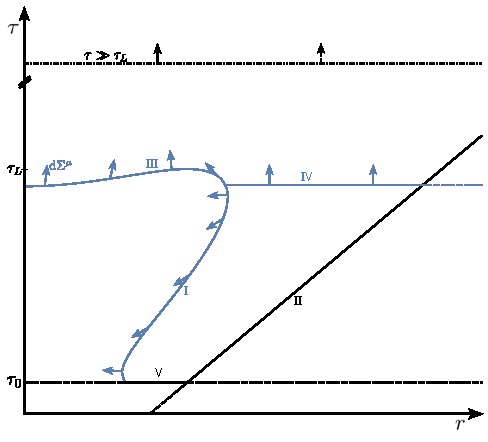
\includegraphics[width=0.4\linewidth]{images/FreezeOutSurface.pdf}
        \captionof{figure}{Freezeout surface in $\tau$-$r$-plane\cite{KirchnerEtAl_2023}.}
        \label{fig:FreezeOutSurface_rtau}
    \end{minipage}
}

Consider the freezeout on the hypersurface depicted in \ref{fig:FreezeOutSurface_rtau}. Assume that the condensate contribution as a function in phase space $f_{\text{cond}}(x^\mu,\vec{p})$ vanishes on $\Sigma_{\text{\rom{2}}}$ and $\Sigma_{\text{\rom{5}}}$, i.e. is contained within the union of all light cones starting on the freeze out surface $\Sigma_{FO}\equiv\Sigma_{\text{\rom{1}}}\cap\Sigma_\text{{\rom{3}}}$. \todo{By causality this seems reasonable, but from Fourier decomposition of a classical field this is not at all clear.}


Following the reasoning from \cite{KirchnerEtAl_2023}, we wish to apply Gauß law. Consider separately the contribution on the $\tau$-axis
\begin{equation*}
    \int_{\Sigma_{r=0}}\dt\Sigma_\mu J^\mu\qquad\text{or}\qquad\lim_{r\to 0}\int_{\Sigma_{r}}\dt\Sigma_\mu J^\mu
\end{equation*}
The surface vector on this hypersurface is $\dt\Sigma_\mu=r\tau\dt\tau\dt\eta\dt\varphi(0,1,0,0)$ and thus vanishes at $r=0$ (the hypersurface $\Sigma_{r=0}$ has zero $3$-volume). Since the derivative in the integrad introduces no divergencies, the contribution of $\Sigma_{r=0}$ to Gauß law is zero.
% \begin{subequations}
%     \begin{align}
%         \partial_\mu=(\partial_t,\partial_x,\partial_y,\partial_z)                                                                                                              \\
%         \partial_x+\partial_y=(\frac{\partial r}{\partial x}+\frac{\partial r}{\partial y})\frac{\partial}{\partial r}                                                          \\
%         \hat{e}_x\partial_x+\hat{e}_y\partial_y=\hat{e}_x\frac{\partial r}{\partial x}\partial_r+\hat{e}_y\frac{\partial r}{\partial y}\partial_r\partial_r=\hat{e}_r\partial_r \\
%         =\cos\varphi\hat{e}_x\partial_r+\sin\varphi\hat{e}_y                                                                                                                    \\
%         \hat{e}_r=\cos\varphi\hat{e}_x+\sin\varphi\hat{e}_y                                                                                                                     \\
%         \hat{e}_\varphi=-\sin\varphi\hat{e}_x+\cos\varphi\hat{e}_y                                                                                                              \\
%         \hat{e}_x=\cos\varphi\hat{e}_r-\sin\varphi\hat{e}_\varphi                                                                                                               \\
%         \hat{e}_y=\sin\varphi\hat{e}_r+\cos\varphi\hat{e}_varphi                                                                                                                \\
%     \end{align}
% \end{subequations}

We can therefore write
\begin{equation}
    \tilde{\phi}(\vec{p})=(\phi,u_{\vec{p}})_{\Sigma_t}=(\phi,u_{\vec{p}})_{\Sigma_{\tau\gg\tau_L}}=(\phi,u_{\vec{p}})_{\Sigma_{FO}}
\end{equation}
The second "$=$" assumes that $\phi=0$ for large spacetime rapidities $\eta\to\pm\infty$ and the $\tau=\const$ hypersurface can be deformed to a $t=\const$ hypersurface.

Using the freezeout surface parametrization stated in earlier paragraphs one computes
\begin{subequations}
    \begin{align}
        \tilde{\phi}(\vec{p}) & =-\imagu\int_{-\infty}^\infty\dt\eta\int_0^{2\pi}\dt\varphi\int_0^\pi\dt\alpha\tau(\alpha) r(\alpha)\frac{1}{\sqrt{2\omega_{\vec{p}}}}\Bigg[r^\prime(\alpha)\phi(\tau,r)\overset{\leftrightarrow}{\partial_\tau}e^{\imagu(\tau \omega_\perp\cosh(\eta-\eta_p)-r p_\perp\cos(\varphi-\varphi_p))}+\nonumber \\
                              & \phantom{=}\qquad + \tau^\prime(\alpha)\phi(\tau,r)\overset{\leftrightarrow}{\partial_r}e^{\imagu(\tau \omega_\perp\cosh(\eta-\eta_p)-r p_\perp\cos(\varphi-\varphi_p))}\Bigg]                                                                                                                             \\
                              & =-\imagu\int_{-\infty}^\infty\dt\eta\int_0^{2\pi}\dt\varphi\int_0^\pi\dt\alpha\tau(\alpha) r(\alpha)\frac{1}{\sqrt{2\omega_{\vec{p}}}}\Bigg[r^\prime(\alpha)\phi(\tau,r)\overset{\leftrightarrow}{\partial_\tau}e^{\imagu(\tau \omega_\perp\cosh\eta-r p_\perp\cos\varphi)}+\nonumber                      \\
                              & \phantom{=}\qquad + \tau^\prime(\alpha)\phi(\tau,r)\overset{\leftrightarrow}{\partial_r}e^{\imagu(\tau \omega_\perp\cosh\eta-r p_\perp\cos\varphi)}\Bigg]                                                                                                                                                  \\
                              & =-\imagu\int_0^\pi\dt\alpha\tau(\alpha) r(\alpha)\frac{1}{\sqrt{2\omega_{\vec{p}}}}\Bigg[r^\prime(\alpha)\phi(\tau,r)\overset{\leftrightarrow}{\partial_\tau}\Big[2\pi J_0(r p_\perp)\times\pi\big(-Y_0(\tau\omega_\perp)+\imagu J_0(\tau\omega_\perp)\big)\Big]+\nonumber                                 \\
                              & \phantom{=}\qquad + \tau^\prime(\alpha)\phi(\tau,r)\overset{\leftrightarrow}{\partial_r}\Big[2\pi J_0(r p_\perp)\times\pi\big(-Y_0(\tau\omega_\perp)+\imagu J_0(\tau\omega_\perp)\big)\Big]\Bigg]                                                                                                          \\
                              & =-\imagu\int_0^\pi\dt\alpha\tau(\alpha) r(\alpha)\frac{1}{\sqrt{2\omega_{\vec{p}}}}\Bigg[-(r^\prime\partial_\tau+\tau^\prime\partial_r)\phi(\tau,r)[2\pi J_0(r p_\perp)\times\pi\big(-Y_0(\tau\omega_\perp)+\imagu J_0(\tau\omega_\perp)\big)\Big]+\nonumber                                               \\
                              & \phantom{=}\qquad + \phi(\tau,r)\Big[\tau^\prime\times2\pi p_\perp J_1(r p_\perp)\times\pi\big(-Y_0(\tau\omega_\perp)+\imagu J_0(\tau\omega_\perp)\big)+\nonumber                                                                                                                                          \\
                              & \phantom{=}\qquad\phantom{-\phi(\tau,r)\Big[}+r^\prime\times2\pi J_0(r p_\perp)\times\pi\omega_\perp\big(Y_1(\tau\omega_\perp)-\imagu J_0(\tau\omega_\perp)\big)\Big]\Bigg]                                                                                                                                \\
                              & =-\frac{2\pi^2\imagu}{\sqrt{2\omega_{\vec{p}}}}\int_0^\pi\dt\alpha\tau(\alpha) r(\alpha)\Bigg[-(r^\prime\partial_\tau+\tau^\prime\partial_r)\phi(\tau,r)[J_0(r p_\perp)\times\big(-Y_0(\tau\omega_\perp)+\imagu J_0(\tau\omega_\perp)\big)\Big]+\nonumber                                                  \\
                              & \phantom{=}\qquad + \phi(\tau,r)\Big[\tau^\prime\times p_\perp J_1(r p_\perp)\times\big(-Y_0(\tau\omega_\perp)+\imagu J_0(\tau\omega_\perp)\big)+\nonumber                                                                                                                                                 \\
                              & \phantom{=}\qquad\phantom{-\phi(\tau,r)\Big[}+r^\prime\times J_0(r p_\perp)\times\omega_\perp\big(Y_1(\tau\omega_\perp)-\imagu J_0(\tau\omega_\perp)\big)\Big]\Bigg]
    \end{align}
\end{subequations}
where the Bessel function identities \eqref{eq:BesselFunctions} were used. One may choose to work at mid-rapidity $\eta_p=0$ where $\omega_{\vec{p}}=m_\perp\vert_{\text{on-shell}}=\omega_\perp$. Note that for large $p_\perp$ one finds
\begin{equation}
    \omega_\perp\sim p_\perp\,,\qquad J_\nu,Y_\nu\sim\frac{1}{\sqrt{p_\perp}}
\end{equation}
and therefore $\phi(\vec{p})\sim\frac{1}{\sqrt{p_\perp}}$.

How to treat the projection $r^\prime\partial_\tau+\tau^\prime\partial_r\equiv\partial_\perp\propto n^\mu\partial_\mu$ of $\partial_\mu$ onto the normal vector $\propto n^\mu$? One could argue that $\partial_\perp\phi$ not specified by field data on the hypersurface and one needs to find suitable initial conditions. A reasonable choice would be $\pi\vert_{\Sigma_{FO}}\equiv\dot{\phi}\vert_{\Sigma_{FO}}=0$. Since $\partial_\eta\phi=0$ by symmetry assumption, this implies $\partial_\tau\phi\vert_{\Sigma_{FO}}=0$. The derivatives $\partial_\alpha\equiv\tau^\prime\partial_\tau+r^\prime\partial_r$ and $\partial_\perp\equiv r^\prime\partial_\tau+\tau^\prime\partial_r$ therefore can be related by $\partial_\perp\phi\vert_{\Sigma_{FO}}=\frac{\tau^\prime}{r^\prime}\partial_\alpha\phi\vert_{\Sigma_{FO}}$.

In the spirit of identifying the pion field with fluid variables, one could argue
\begin{equation}
    \partial_\mu\phi=\partial_\mu(\rho\exp(\imagu\vartheta))=\imagu\phi\partial_\mu\vartheta=\imagu\phi\chi u_\mu
\end{equation}

Really we are only interested in the pionic component of $\phi$, which by definition is $\pi=\sqrt{2}\Im\phi$. Replace all $\phi$'s in the last paragraph by $\pi$ maybe? Yes, real and imaginary part fulfill the homogeneous KG equation separately. It's derivative is
\begin{equation}
    \partial_\mu\pi=\sqrt{2}\Im\partial_\mu\phi=\sqrt{2}\chi u_\mu\Re\phi=\sigma\chi u_\mu
\end{equation}
